%
% strukturen.tex
%
% (c) 2021 Prof Dr Andreas Müller, OST Ostschweizer Fachhochschule
%
\begin{frame}[t]
\frametitle{Strukturen}
\vspace{-15pt}
\begin{columns}[t,onlytextwidth]
\begin{column}{0.42\textwidth}
\begin{center}
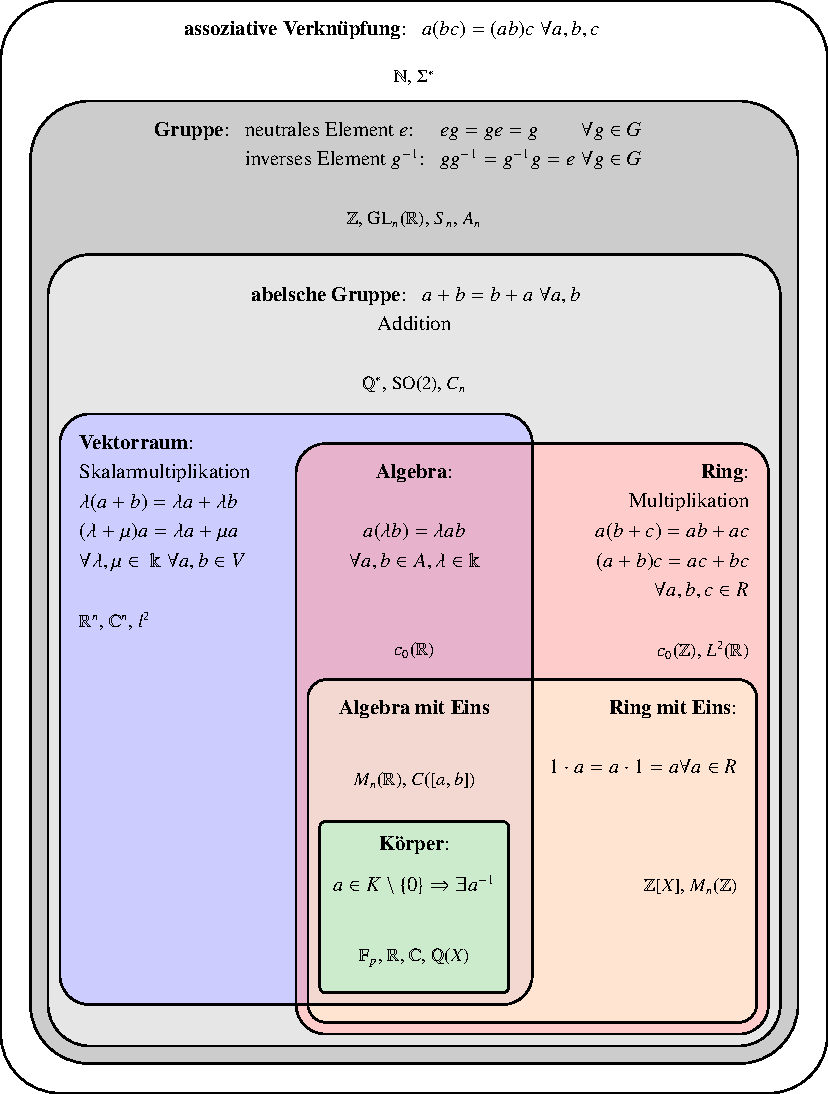
\includegraphics[width=\textwidth]{../../buch/chapters/10-vektorenmatrizen/images/strukturen.pdf}
\end{center}
\end{column}
\begin{column}{0.54\textwidth}
\begin{itemize}[<+->]
\item Gruppen: Drehungen, Symmetrien
\item Vektorraum: Geometrie
\item Ring (mit Eins)
\item Algebra: Vektorraum und Ring
\item Algebra mit Eins: Vektorraum und Ring mit Eins
\item Körper
\end{itemize}
\uncover<7->{%
\begin{block}{Matrizen}
Jede beliebige Struktur lässt sich mit Matrizen darstellen:
\begin{itemize}
\item<8-> Permutationsmatrizen
\item<9-> Wahrscheinlichkeitsmatrizen
\item<10-> Wurzeln
\end{itemize}
\end{block}}
\end{column}
\end{columns}
\end{frame}
